\documentclass[
11pt, % The default document font size, options: 10pt, 11pt, 12pt
%codirector, % Uncomment to add a codirector to the title page
]{charter} 


% El títulos de la memoria, se usa en la carátula y se puede usar el cualquier lugar del documento con el comando \ttitle
\titulo{Control nutricional basado en IA} 

% Nombre del posgrado, se usa en la carátula y se puede usar el cualquier lugar del documento con el comando \degreename
\posgrado{Carrera de Especialización en Inteligencia Artificial}

% Tu nombre, se puede usar el cualquier lugar del documento con el comando \authorname
% IMPORTANTE: no omitir titulaciones ni tildación en los nombres, también se recomienda escribir los nombres completos (tal cual los tienen en su documento)
% Nombre y director definidos directamente en charter.cls para evitar referencias circulares
%\autor{\authorname}

% El nombre del director y co-director, se puede usar el cualquier lugar del documento con el comando \supname y \cosupname y \pertesupname y \pertecosupname
%\director{\supname}
%\pertenenciaDirector{pertenencia}
%\codirector{\cosupname} % para que aparezca en la portada se debe descomentar la opción codirector en los parámetros de documentclass
%\pertenenciaCoDirector{FIUBA}

% Nombre del cliente, quien va a aprobar los resultados del proyecto, se puede usar con el comando \clientename y \empclientename
%\cliente{Nombre del cliente}
%\empresaCliente{Empresa del cliente}
 
\fechaINICIO{3 de marzo de 2026}		%Fecha de inicio de la cursada de GdP \fechaInicioName
\fechaFINALPlan{21 de abril de 2026} 	%Fecha de final de cursada de GdP
% \fechaFINALTrabajo{15 de mayo de 2024}	%Fecha de defensa pública del trabajo final


\begin{document}

\maketitle
\thispagestyle{empty}
\pagebreak


\thispagestyle{empty}
{\setlength{\parskip}{0pt}
\tableofcontents{}
}
\pagebreak


\section*{Registros de cambios}
\label{sec:registro}


\begin{table}[ht]
\label{tab:registro}
\centering
\begin{tabularx}{\linewidth}{@{}|c|X|c|@{}}
\hline
\rowcolor[HTML]{C0C0C0} 
Revisión & \multicolumn{1}{c|}{\cellcolor[HTML]{C0C0C0}Detalles de los cambios realizados} & Fecha      \\ \hline
0      & Creación del documento                                 &\fechaInicioName \\ \hline
1      & Se completa hasta el punto 5 inclusive                & 15 de marzo de 2026 \\ \hline
%2      & Se completa hasta el punto 9 inclusive
%		  Se puede agregar algo más \newline
%		  En distintas líneas \newline
%		  Así                                                    & {día} de {mes} de 202X \\ \hline
%3      & Se completa hasta el punto 12 inclusive                & {día} de {mes} de 202X \\ \hline
%4      & Se completa el plan	                                 & {día} de {mes} de 202X \\ \hline

% Si hay más correcciones pasada la versión 4 también se deben especificar acá

\end{tabularx}
\end{table}

\pagebreak



\section*{Acta de constitución del proyecto}
\label{sec:acta}

\begin{flushright}
Buenos Aires, \fechaInicioName
\end{flushright}

\vspace{2cm}

Por medio de la presente se acuerda con el \authorname\hspace{1px} que su Trabajo Final de la \degreename\hspace{1px} se titulará ``\ttitle'' y consistirá en el desarrollo de un prototipo de aplicación móvil que utiliza visión por computadora e inteligencia artificial para analizar fotografías de alimentos, identificar sus componentes, estimar porciones y generar registros nutricionales automáticos. El trabajo tendrá un presupuesto preliminar estimado de 600 horas y un costo estimado de \textcolor{red}{\$ XXX}, con fecha de inicio el \fechaInicioName\hspace{1px} y fecha de presentación pública el \fechaFinalName.

Se adjunta a esta acta la planificación inicial.

\vfill

% Esta parte se construye sola con la información que hayan cargado en el preámbulo del documento y no debe modificarla
\begin{table}[ht]
\centering
\begin{tabular}{ccc}
\begin{tabular}[c]{@{}c@{}}Dr. Ing. Ariel Lutenberg \\ Director posgrado FIUBA\end{tabular} & \hspace{2cm} & \begin{tabular}[c]{@{}c@{}}\clientename \\ \empclientename \end{tabular} \vspace{2.5cm} \\ 
\multicolumn{3}{c}{\begin{tabular}[c]{@{}c@{}} \supname \\ Director del Trabajo Final\end{tabular}} \vspace{2.5cm} \\
\end{tabular}
\end{table}




\section{1. Descripción técnica-conceptual del proyecto a realizar}
\label{sec:descripcion}

El seguimiento nutricional es una herramienta fundamental en el tratamiento de enfermedades metabólicas, obesidad y otros trastornos relacionados con la alimentación. Sin embargo, los métodos tradicionales, como el diario de comidas manual, recordatorio de 24 horas o cuestionario de frecuencia alimentaria— presentan limitaciones bien documentadas: subestimación sistemática de la ingesta calórica, sesgo de reporte asociado al peso corporal, y baja adherencia sostenida en el tiempo. Estudios de revisión sistemática concluyen que todos estos instrumentos tienen sesgos inherentes que comprometen su validez clínica~\cite{dahl2020traditional}. En intervenciones de pérdida de peso basadas en aplicaciones móviles, la adherencia al registro cae por debajo del 50\% de los participantes ya en la semana 10~\cite{lyzwinski2019adherence}, y el tiempo requerido para el registro alcanza aproximadamente 23 minutos diarios durante el primer mes~\cite{vitale2022burden}.

Aplicaciones como MyFitnessPal, Cronometer o Noom han digitalizado parcialmente el proceso, pero siguen dependiendo del ingreso manual de alimentos mediante búsqueda en base de datos, lo que conserva la mayor parte de la fricción original. El reconocimiento automático de alimentos a partir de imágenes representa una alternativa de mayor potencial. Desde el trabajo pionero de Myers et al.~\cite{myers2015im2calories} (Im2Calories, Google, ICCV 2015), que demostró la factibilidad de estimar calorías a partir de una fotografía tomada con un teléfono, el campo ha avanzado considerablemente. Modelos basados en redes convolucionales (CNN) como DeepFood~\cite{liu2016deepfood} alcanzaron un 77,4\% de exactitud \textit{top-1} en Food-101, el conjunto de datos de referencia más utilizado (101.000 imágenes, 101 categorías). Con la adopción de Vision Transformers (ViT) y técnicas de aumento de datos, los modelos recientes superan el 91\% en el mismo benchmark~\cite{mdpi2025review}, y arquitecturas como NoisyViT reportan hasta 99,5\% en condiciones de laboratorio.

No obstante, existe una brecha significativa entre el desempeño en benchmarks controlados y el rendimiento en entornos reales. La validación clínica de la aplicación CALO mama~\cite{nakamura2022calomama} mostró que el sistema estimaba correctamente solo 11 de 30 nutrientes evaluados; y un análisis comparativo de 18 aplicaciones comerciales~\cite{nutrients2024review} encontró que los sistemas de IA subestiman sistemáticamente platos de cocinas no occidentales. Dos desafíos técnicos dominan el estado del arte: la \textbf{ambigüedad de escala} en imágenes monoculares —sin referencia física no es posible determinar el tamaño real del plato— y la \textbf{oclusión} en preparaciones mixtas. Los errores en la estimación de volumen de porciones oscilan entre el 10\% y el 33\% de error relativo~\cite{martinezgarcia2023}. Trabajos recientes como MFP3D~\cite{mfp3d2024} abordan este problema mediante reconstrucción de nubes de puntos 3D a partir de imágenes monoculares, mientras que DietAI24~\cite{dietai24_2025} propone integrar modelos de lenguaje multimodal con bases de datos nutricionales para estimar hasta 65 nutrientes desde fotografías.

Este proyecto propone el desarrollo de un prototipo de aplicación móvil que utiliza visión por computadora e inteligencia artificial para analizar imágenes de platos de comida, identificar sus componentes, estimar porciones e integrar los datos nutricionales de forma automática. La solución está orientada a dos perfiles complementarios: el paciente en seguimiento nutricional, que obtiene un registro preciso con mínimo esfuerzo; y el profesional de la nutrición, que accede a datos objetivos para orientar el tratamiento. Se trata de un proyecto personal enmarcado en la Carrera de Especialización en Inteligencia Artificial de la FIUBA, sin vinculación empresarial ni financiamiento externo. El prototipo se ubica en una etapa temprana del ciclo de vida, con foco en validar la factibilidad técnica del enfoque propuesto para el contexto local.

En la figura \ref{fig:diagBloques} se presenta el diagrama en bloques del sistema. El flujo comienza con la captura de una fotografía por parte del usuario a través de la aplicación móvil. La imagen es procesada por un módulo de visión por computadora que detecta e identifica los componentes alimentarios presentes en el plato. Un módulo de estimación de porciones infiere las cantidades a partir de referencias visuales. Con esos datos se consulta una base de datos nutricional para obtener los macronutrientes correspondientes —calorías, proteínas, grasas y carbohidratos— y se genera un registro dietético disponible para el paciente y, en etapas futuras, para el profesional tratante.

\begin{figure}[htpb]
\centering
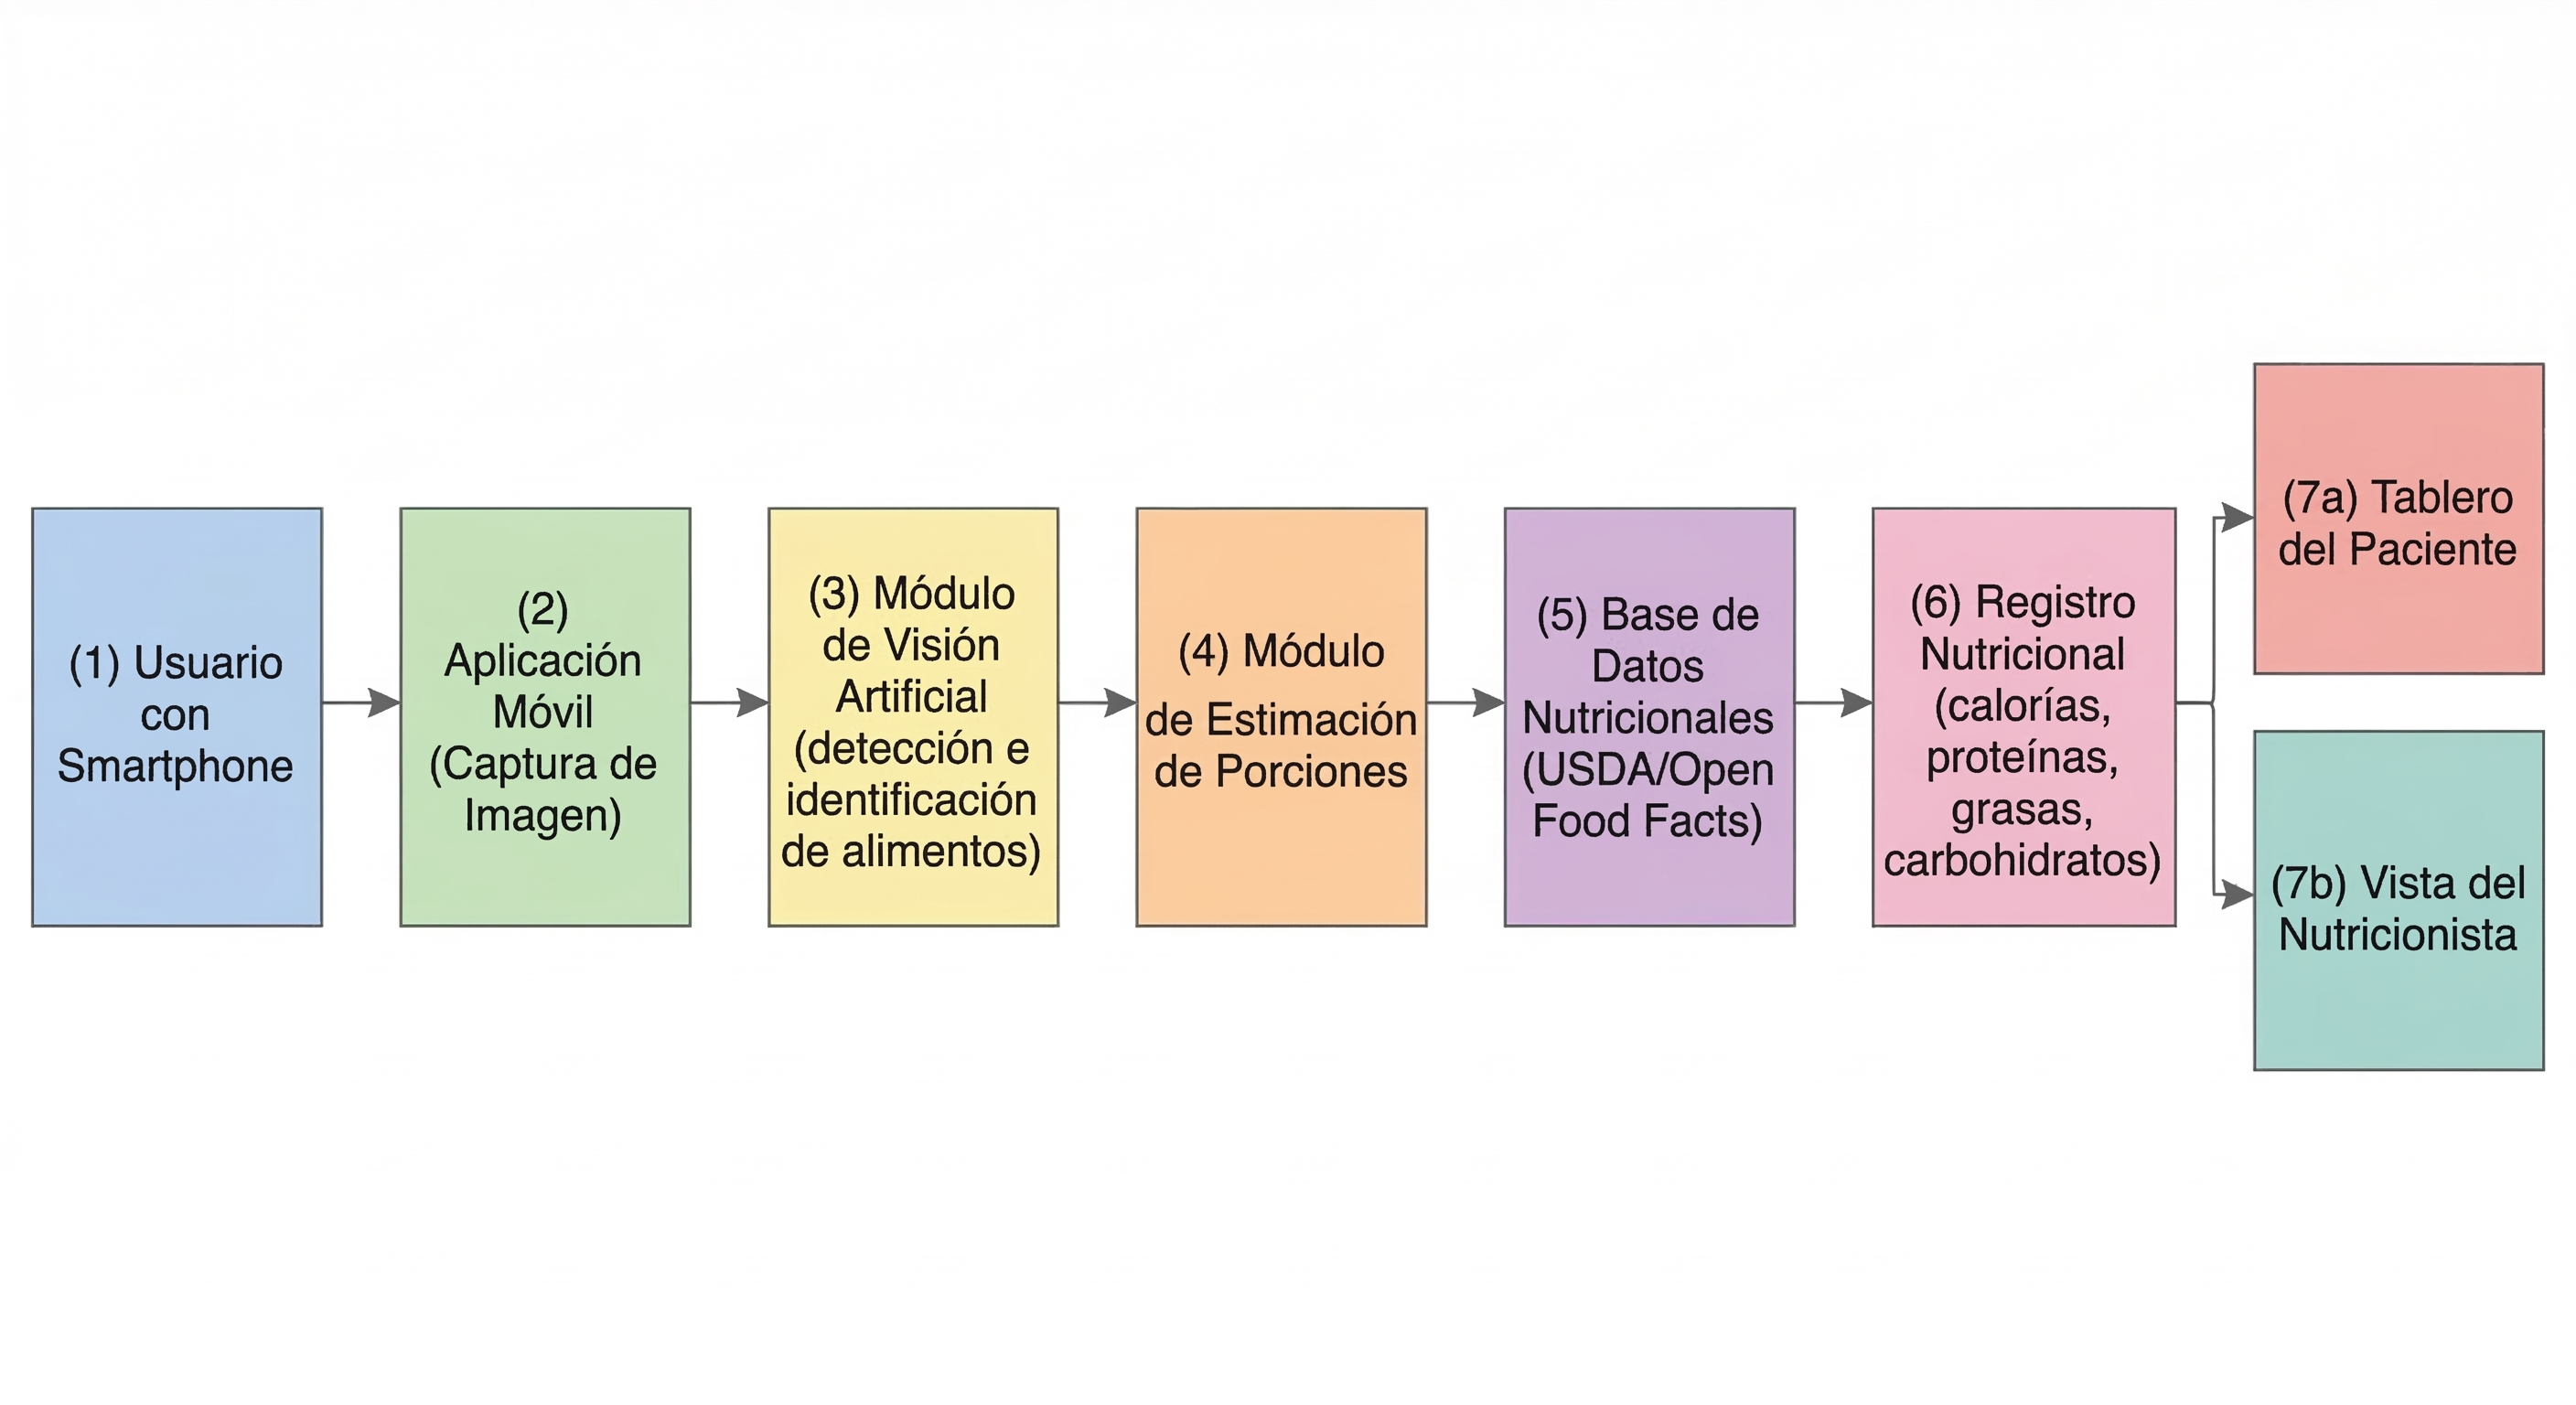
\includegraphics[width=.65\textwidth]{./Figuras/diagBloques.png}
\caption{Diagrama en bloques del sistema.}
\label{fig:diagBloques}
\end{figure}

\section{2. Identificación y análisis de los interesados}
\label{sec:interesados}

\begin{table}[ht]
\begin{tabularx}{\linewidth}{@{}|l|X|X|l|@{}}
\hline
\rowcolor[HTML]{C0C0C0}
Rol           & Nombre y Apellido                                                  & Organización                          & Puesto                      \\ \hline
Responsable   & \authorname                                                        & Independiente                         & Alumno CEIA--FIUBA           \\ \hline
Orientador    & \supname                                                           & \pertesupname                         & Director del Trabajo Final  \\ \hline
Usuario final & Personas en seguimiento nutricional                                & -                                     & -                           \\ \hline
Interesado    & Licenciados en Nutrición y Dietistas \newline (AADYND / AALeN)     & Asoc. Argentina de Dietistas y Lic. en Nutrición & -              \\ \hline
Interesado    & Profesionales de Diabetología                                      & Sociedad Argentina de Diabetes (SAD)  & -                           \\ \hline
Interesado    & Profesionales de Obesidad y Trastornos Alimentarios                & Soc. Argentina de Obesidad y Trast. Alimentarios (SAOTA) & - \\ \hline
Opositor      & Aplicaciones de registro nutricional manual                        & MyFitnessPal, Cronometer, entre otras & -                           \\ \hline
\end{tabularx}
\end{table}

\begin{itemize}
	\item Responsable: \authorname{} es el único miembro del equipo de desarrollo. Gestiona, diseña e implementa el sistema en el marco de la Carrera de Especialización en Inteligencia Artificial de la FIUBA, como profesional independiente sin vinculación institucional.
	\item Orientador: El \supname{} orienta la definición de los requerimientos del sistema, la selección de enfoques técnicos y la evaluación de los resultados del Trabajo Final.
	\item Usuario final: personas que siguen un plan nutricional y necesitan registrar su ingesta alimentaria de manera precisa y sin fricción. Es el beneficiario primario de la solución.
	\item Interesado (AADYND / AALeN): la Asociación Argentina de Dietistas y Licenciados en Nutrición agrupa a los profesionales que podrían adoptar la herramienta como complemento en sus prácticas clínicas, o participar en la validación de los registros nutricionales generados.
	\item Interesado (SAD): la Sociedad Argentina de Diabetes representa a profesionales y pacientes para quienes el control dietético es crítico en el manejo de la enfermedad. Constituye un potencial adoptante institucional en fases avanzadas del producto.
	\item Interesado (SAOTA): la Sociedad Argentina de Obesidad y Trastornos Alimentarios es el nexo entre profesionales y pacientes en el tratamiento de la obesidad, condición en la que el monitoreo calórico es un componente central del protocolo terapéutico. Podría actuar como validador clínico del sistema.
	\item Opositor: las aplicaciones de registro manual existentes (MyFitnessPal, Cronometer) tienen bases de usuarios establecidas y podrían representar resistencia al cambio, tanto por parte de los usuarios como de los profesionales que ya las recomiendan en sus consultas.
\end{itemize}


\section{3. Propósito del proyecto}
\label{sec:proposito}

Facilitar el registro nutricional preciso y de baja fricción mediante inteligencia artificial y visión por computadora, reduciendo la carga cognitiva que representa el seguimiento manual para el paciente y proveyendo a los profesionales de la salud información objetiva que mejore la calidad del acompañamiento dietético.

\section{4. Alcance del proyecto}
\label{sec:alcance}

El proyecto incluye:

\begin{itemize}
	\item Relevamiento del estado del arte en reconocimiento de alimentos y estimación de porciones mediante visión por computadora.
	\item Recolección y preparación de un conjunto de datos de imágenes de alimentos etiquetado, adecuado para el entrenamiento y evaluación de los modelos.
	\item Desarrollo y entrenamiento de un modelo de visión por computadora para la detección e identificación de componentes alimentarios en fotografías.
	\item Desarrollo de un módulo de estimación de porciones a partir de imágenes.
	\item Integración con una base de datos nutricional de acceso público para la consulta de macronutrientes (calorías, proteínas, grasas y carbohidratos).
	\item Desarrollo de un prototipo de aplicación móvil que integre los módulos anteriores, permitiendo al usuario fotografiar su comida y obtener un registro nutricional automático.
	\item Documentación técnica del sistema y memoria del Trabajo Final.
\end{itemize}

El presente proyecto no incluye:

\begin{itemize}
	\item El despliegue en producción ni la publicación en tiendas de aplicaciones (App Store o Google Play).
	\item El desarrollo de funcionalidades específicas para profesionales de la nutrición (portal clínico, prescripción de dietas, gestión de pacientes).
	\item La integración con sistemas de gestión clínica (HIS/EHR).
	\item El soporte multilingüe; el sistema operará exclusivamente en español.
	\item El desarrollo de un modelo de negocio o funcionalidades de monetización.
	\item La evaluación clínica formal con pacientes reales.
\end{itemize}


\section{5. Supuestos del proyecto}
\label{sec:supuestos}

Para el desarrollo del presente proyecto se supone que:

\begin{itemize}
	\item El alumno dispondrá de al menos 15 horas semanales para dedicar al proyecto durante su desarrollo.
	\item Es técnicamente posible estimar porciones de alimentos a partir de imágenes monoculares con un margen de error aceptable para uso en seguimiento nutricional no clínico.
	\item Los \textit{datasets} públicos de imágenes de alimentos disponibles (como Food-101 u Open Images) son suficientemente representativos de los alimentos del contexto local para entrenar modelos con precisión aceptable.
	\item Las bases de datos nutricionales de acceso público (como USDA FoodData Central u Open Food Facts) contienen datos suficientes para cubrir los alimentos más comunes de la dieta argentina.
	\item El hardware disponible —computadora personal con GPU o acceso a plataformas de cómputo en la nube como Google Colab— será suficiente para el entrenamiento de los modelos requeridos.
	\item Los usuarios finales disponen de un \textit{smartphone} con cámara de resolución adecuada y acceso a internet.
	\item El prototipo no requerirá aprobaciones regulatorias durante la etapa de investigación académica.
\end{itemize}

\section{6. Requerimientos}
\label{sec:requerimientos}

\begin{consigna}{red} % ELIMINAR \begin{consigna}{red} y \end{consigna}{red} en las secciones que vayan completando para cada entrega parcial.
Los requerimientos deben enumerarse y de ser posible estar agrupados por afinidad, por ejemplo:

\begin{enumerate}
	\item Requerimientos funcionales:
		\begin{enumerate}
			\item El sistema debe...
			\item Tal componente debe...
			\item El usuario debe poder...
		\end{enumerate}
	\item Requerimientos de documentación:
		\begin{enumerate}
			\item Requerimiento 1.
			\item Requerimiento 2 (prioridad menor)
		\end{enumerate}
	\item Requerimiento de testing...
	\item Requerimientos de la interfaz...
	\item Requerimientos interoperabilidad...
	\item etc...
\end{enumerate}

Leyendo los requerimientos se debe poder interpretar cómo será el proyecto y su funcionalidad.

Indicar claramente cuál es la prioridad entre los distintos requerimientos y si hay requerimientos opcionales. 

\textbf{¡¡¡No olvidarse de que los requerimientos incluyen a las regulaciones y normas vigentes!!!}

Y al escribirlos seguir las siguientes reglas:
\begin{itemize}
	\item Ser breve y conciso (nadie lee cosas largas). 
	\item Ser específico: no dejar lugar a confusiones.
	\item Expresar los requerimientos en términos que sean cuantificables y medibles.
\end{itemize}

\end{consigna} % ELIMINAR \begin{consigna}{red} y \end{consigna}{red} en las secciones que vayan completando para cada entrega parcial.

\section{7. Historias de usuarios (\textit{Product backlog})}
\label{sec:backlog}

\begin{consigna}{red}
Descripción: en esta sección se deben incluir las historias de usuarios y su ponderación (\textit{history points}). Recordar que las historias de usuarios son descripciones cortas y simples de una característica contada desde la perspectiva de la persona que desea la nueva capacidad, generalmente un usuario o cliente del sistema. La ponderación es un número entero que representa el tamaño de la historia comparada con otras historias de similar tipo.

Se debe indicar explícitamente el criterio para calcular los \textit{story points} de cada historia.

El formato propuesto es: 
\begin{enumerate}
\item ``Como [rol] quiero [tal cosa] para [tal otra cosa]."

\textit{Story points}: 8 (complejidad: 3, dificultad: 2, incertidumbre: 3)
\end{enumerate}
\end{consigna}

\section{8. Entregables principales del proyecto}
\label{sec:entregables}

\begin{consigna}{red}
Los entregables del proyecto son (ejemplo):

\begin{itemize}
	\item Manual de usuario.
	\item Diagrama de circuitos esquemáticos.
	\item Código fuente del firmware.
	\item Diagrama de instalación.
	\item Memoria del trabajo final.
	\item etc...
\end{itemize}
\end{consigna}

\section{9. Desglose del trabajo en tareas}
\label{sec:wbs}

\begin{consigna}{red}
El WBS debe tener relación directa o indirecta con los requerimientos.  Son todas las actividades que se harán en el proyecto para dar cumplimiento a los requerimientos. Se recomienda mostrar el WBS mediante una lista indexada:

\begin{enumerate}
\item Grupo de tareas 1 (suma h)
	\begin{enumerate}
	\item Tarea 1 (tantas h)
	\item Tarea 2 (tantas h)
	\item Tarea 3 (tantas h)
	\end{enumerate}
\item Grupo de tareas 2 (suma h)
	\begin{enumerate}
	\item Tarea 1 (tantas h)
	\item Tarea 2 (tantas h)
	\item Tarea 3 (tantas h)
	\end{enumerate}
\item Grupo de tareas 3 (suma h)
	\begin{enumerate}
	\item Tarea 1 (tantas h)
	\item Tarea 2 (tantas h)
	\item Tarea 3 (tantas h)
	\item Tarea 4 (tantas h)
	\item Tarea 5 (tantas h)
	\end{enumerate}
\end{enumerate}

Cantidad total de horas: tantas.

\textbf{¡Importante!:} la unidad de horas es h y va separada por espacio del número. Es incorrecto escribir ``23hs".

\textbf{Se recomienda que no haya ninguna tarea que lleve más de 40 h.} De ser así se recomienda dividirla en tareas de menor duración.

\end{consigna}

\section{10. Diagrama de Activity On Node}
\label{sec:AoN}

\begin{consigna}{red}
Armar el AoN a partir del WBS definido en la etapa anterior.

Una herramienta simple para desarrollar los diagramas es el Draw.io (\url{https://app.diagrams.net/}).
\href{https://app.diagrams.net}{Draw.io}


\begin{figure}[htpb]
\centering 
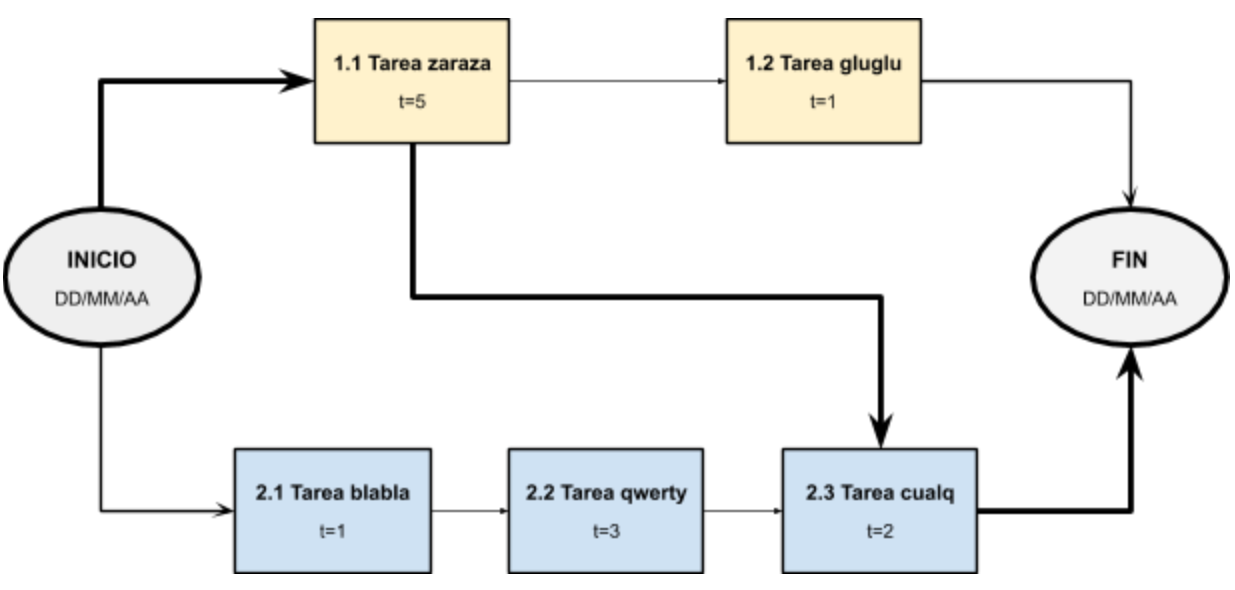
\includegraphics[width=.8\textwidth]{./Figuras/AoN.png}
\caption{Diagrama de \textit{Activity on Node}.}
\label{fig:AoN}
\end{figure}

Indicar claramente en qué unidades están expresados los tiempos.
De ser necesario indicar los caminos semi críticos y analizar sus tiempos mediante un cuadro.
Es recomendable usar colores y un cuadro indicativo describiendo qué representa cada color.

\end{consigna}

\section{11. Diagrama de Gantt}
\label{sec:gantt}

\begin{consigna}{red}
Existen muchos programas y recursos \textit{online} para hacer diagramas de Gantt, entre los cuales destacamos:

\begin{itemize}
\item Planner
\item GanttProject
\item Trello + \textit{plugins}. En el siguiente link hay un tutorial oficial: \\ \url{https://blog.trello.com/es/diagrama-de-gantt-de-un-proyecto}
\item Creately, herramienta online colaborativa. \\\url{https://creately.com/diagram/example/ieb3p3ml/LaTeX}
\item Se puede hacer en latex con el paquete \textit{pgfgantt}\\ \url{http://ctan.dcc.uchile.cl/graphics/pgf/contrib/pgfgantt/pgfgantt.pdf}
\end{itemize}

Pegar acá una captura de pantalla del diagrama de Gantt, cuidando que la letra sea suficientemente grande como para ser legible. 
Si el diagrama queda demasiado ancho, se puede pegar primero la ``tabla'' del Gantt y luego pegar la parte del diagrama de barras del diagrama de Gantt.

Configurar el software para que en la parte de la tabla muestre los códigos del EDT (WBS).\\
Configurar el software para que al lado de cada barra muestre el nombre de cada tarea.\\
Revisar que la fecha de finalización coincida con lo indicado en el Acta Constitutiva.

En la figura \ref{fig:gantt}, se muestra un ejemplo de diagrama de gantt realizado con el paquete de \textit{pgfgantt}. 
En la plantilla pueden ver el código que lo genera y usarlo de base para construir el propio.

Las fechas pueden ser calculadas utilizando alguna de las herramientas antes citadas. Sin embargo, el siguiente ejemplo
fue elaborado utilizando 
\href{https://docs.google.com/spreadsheets/d/1fBz8NhSpc4tkkhz3KjJCbh1nR_ltDkfEcZi4tZXduqs}{esta hoja de cálculo}.

Es importante destacar que el ancho del diagrama estará dado por la longitud del texto utilizado para las tareas 
(Ejemplo: tarea 1, tarea 2, etcétera) y el valor \textit{x unit}. Para mejorar la apariencia del diagrama, es necesario
ajustar este valor y, quizás, acortar los nombres de las tareas.

\begin{figure}[htpb]
  \begin{center}
    \begin{ganttchart}[
      time slot unit=day,
      time slot format=isodate,
      x unit=0.038cm,
      y unit title=0.7cm,
      y unit chart=0.6cm,
      milestone/.append style={xscale=4}
      ]{2021-03-05}{2021-12-16}
      \gantttitlecalendar*{2021-03-05}{2021-12-16}{year} \\
      \gantttitlecalendar*{2021-03-05}{2021-12-16}{month} \\
      \ganttgroup{Duración Total}{2021-03-05}{2021-12-16} \\
      %%%%%%%%%%%%%%%%%Organización
      \ganttgroup{Organización}{2021-03-05}{2021-04-16} \\
      \ganttbar{Planificación del proyecto}{2021-03-05}{2021-04-15} \\
      %%%%%%%%%%%%%%%%%Ejecución
      \ganttgroup{Ejecución}{2021-04-16}{2021-10-21} \\
      \ganttbar{Tarea 1}{2021-04-16}{2021-04-29} \\
      \ganttbar{Tarea 2}{2021-04-30}{2021-05-13} \\
      \ganttbar{Tarea 3}{2021-05-14}{2021-05-27} \\
      \ganttbar{Tarea 4}{2021-05-28}{2021-07-12} \\
      \ganttbar{Tarea 5}{2021-07-13}{2021-08-09} \\
      \ganttbar{Tarea 6}{2021-08-10}{2021-09-23} \\
      \ganttbar{Tarea 7}{2021-09-24}{2021-09-30} \\
      \ganttbar{Tarea 8}{2021-10-01}{2021-10-14} \\
      \ganttbar{Tarea 9}{2021-10-15}{2021-10-21} \\
      % %%%%%%%%%%%%%%%%%Finalización
      \ganttgroup{Finalización}{2021-10-22}{2021-12-16} \\
      \ganttbar{Memoria v1}{2021-10-22}{2021-11-04} \\
      \ganttbar{Memoria v2}{2021-11-05}{2021-11-18} \\
      \ganttbar{Memoria final}{2021-11-19}{2021-12-02} \\
      % La fecha del siguiente milestone es la fecha en que terminamos la memoria
      \ganttmilestone{Enviar memoria al director}{2021-12-02} \\
      \ganttbar{Elaborar la presentación}{2021-12-03}{2021-12-16} \\
      \ganttmilestone{Ensayo de la presentación}{2021-12-16} \\
      %%%%%%%%%%%%%%%%%%%%%%%%%%%%%%%%%%%%%%%%%%%%%%%%%%%%%%%%%%%%%%%
    \end{ganttchart}
  \end{center}
  \caption{Diagrama de gantt de ejemplo}
  \label{fig:gantt}
\end{figure}


\begin{landscape}
\begin{figure}[htpb]
\centering 
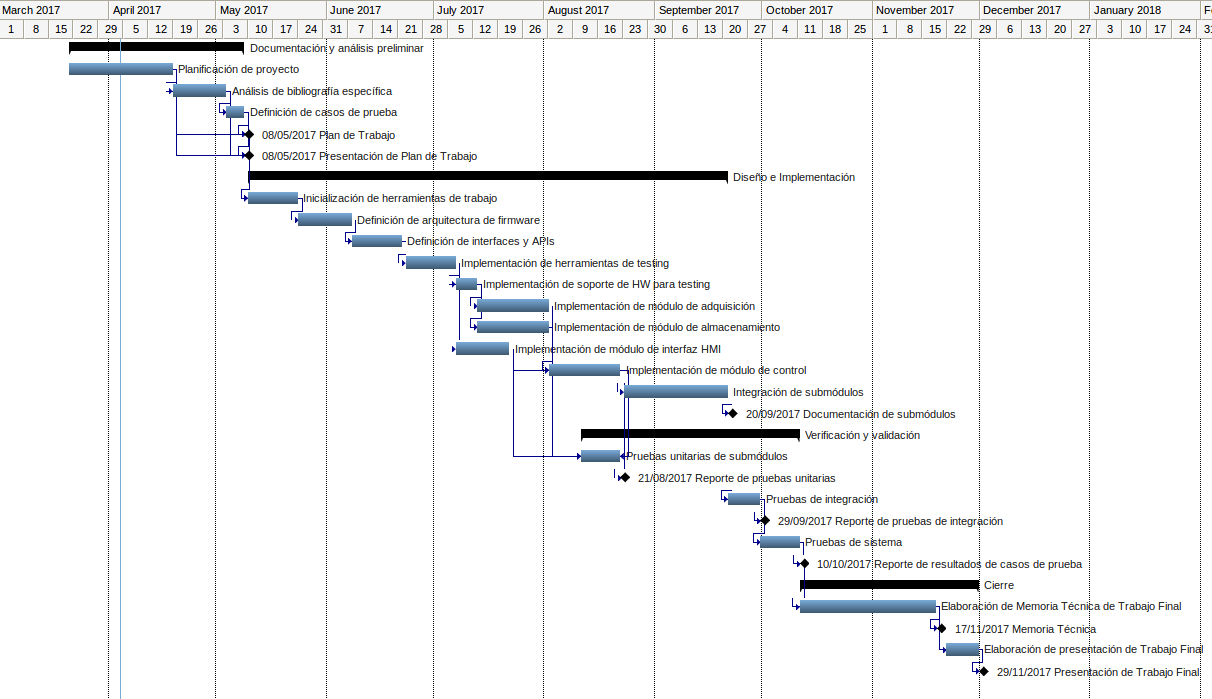
\includegraphics[height=.85\textheight]{./Figuras/Gantt-2.png}
\caption{Ejemplo de diagrama de Gantt (apaisado).} %Modificar este título acorde.
\label{fig:diagGantt}
\end{figure}

\end{landscape}

\end{consigna}


\section{12. Presupuesto detallado del proyecto}
\label{sec:presupuesto}

\begin{consigna}{red}
Si el proyecto es complejo entonces separarlo en partes:
\begin{itemize}
	\item Un total global, indicando el subtotal acumulado por cada una de las áreas.
	\item El desglose detallado del subtotal de cada una de las áreas.
\end{itemize}

IMPORTANTE: No olvidarse de considerar los COSTOS INDIRECTOS.

Incluir la aclaración de si se emplea como moneda el peso argentino (ARS) o si se usa moneda extranjera (USD, EUR, etc). Si es en moneda extranjera se debe indicar la tasa de conversión respecto a la moneda local en una fecha dada.

\end{consigna}

\begin{table}[htpb]
\centering
\begin{tabularx}{\linewidth}{@{}|X|c|r|r|@{}}
\hline
\rowcolor[HTML]{C0C0C0} 
\multicolumn{4}{|c|}{\cellcolor[HTML]{C0C0C0}COSTOS DIRECTOS} \\ \hline
\rowcolor[HTML]{C0C0C0} 
Descripción &
  \multicolumn{1}{c|}{\cellcolor[HTML]{C0C0C0}Cantidad} &
  \multicolumn{1}{c|}{\cellcolor[HTML]{C0C0C0}Valor unitario} &
  \multicolumn{1}{c|}{\cellcolor[HTML]{C0C0C0}Valor total} \\ \hline
 &
  \multicolumn{1}{c|}{} &
  \multicolumn{1}{c|}{} &
  \multicolumn{1}{c|}{} \\ \hline
 &
  \multicolumn{1}{c|}{} &
  \multicolumn{1}{c|}{} &
  \multicolumn{1}{c|}{} \\ \hline
\multicolumn{1}{|l|}{} &
   &
   &
   \\ \hline
\multicolumn{1}{|l|}{} &
   &
   &
   \\ \hline
\multicolumn{3}{|c|}{SUBTOTAL} &
  \multicolumn{1}{c|}{} \\ \hline
\rowcolor[HTML]{C0C0C0} 
\multicolumn{4}{|c|}{\cellcolor[HTML]{C0C0C0}COSTOS INDIRECTOS} \\ \hline
\rowcolor[HTML]{C0C0C0} 
Descripción &
  \multicolumn{1}{c|}{\cellcolor[HTML]{C0C0C0}Cantidad} &
  \multicolumn{1}{c|}{\cellcolor[HTML]{C0C0C0}Valor unitario} &
  \multicolumn{1}{c|}{\cellcolor[HTML]{C0C0C0}Valor total} \\ \hline
\multicolumn{1}{|l|}{} &
   &
   &
   \\ \hline
\multicolumn{1}{|l|}{} &
   &
   &
   \\ \hline
\multicolumn{1}{|l|}{} &
   &
   &
   \\ \hline
\multicolumn{3}{|c|}{SUBTOTAL} &
  \multicolumn{1}{c|}{} \\ \hline
\rowcolor[HTML]{C0C0C0}
\multicolumn{3}{|c|}{TOTAL} &
   \\ \hline
\end{tabularx}%
\end{table}


\section{13. Gestión de riesgos}
\label{sec:riesgos}

\begin{consigna}{red}
a) Identificación de los riesgos (al menos cinco) y estimación de sus consecuencias:
 
Riesgo 1: detallar el riesgo (riesgo es algo que si ocurre altera los planes previstos de forma negativa)
\begin{itemize}
	\item Severidad (S): mientras más severo, más alto es el número (usar números del 1 al 10).\\
	Justificar el motivo por el cual se asigna determinado número de severidad (S).
	\item Probabilidad de ocurrencia (O): mientras más probable, más alto es el número (usar del 1 al 10).\\
	Justificar el motivo por el cual se asigna determinado número de (O). 
\end{itemize}   

Riesgo 2:
\begin{itemize}
	\item Severidad (S): X.\\
	Justificación...
	\item Ocurrencia (O): Y.\\
	Justificación...
\end{itemize}

Riesgo 3:
\begin{itemize}
	\item Severidad (S):  X.\\
	Justificación...
	\item Ocurrencia (O): Y.\\
	Justificación...
\end{itemize}


b) Tabla de gestión de riesgos:      (El RPN se calcula como RPN=SxO)

\begin{table}[htpb]
\centering
\begin{tabularx}{\linewidth}{@{}|X|c|c|c|c|c|c|@{}}
\hline
\rowcolor[HTML]{C0C0C0} 
Riesgo & S & O & RPN & S* & O* & RPN* \\ \hline
       &   &   &     &    &    &      \\ \hline
       &   &   &     &    &    &      \\ \hline
       &   &   &     &    &    &      \\ \hline
       &   &   &     &    &    &      \\ \hline
       &   &   &     &    &    &      \\ \hline
\end{tabularx}%
\end{table}

Criterio adoptado: 

Se tomarán medidas de mitigación en los riesgos cuyos números de RPN sean mayores a...

Nota: los valores marcados con (*) en la tabla corresponden luego de haber aplicado la mitigación.

c) Plan de mitigación de los riesgos que originalmente excedían el RPN máximo establecido:
 
Riesgo 1: plan de mitigación (si por el RPN fuera necesario elaborar un plan de mitigación).
  Nueva asignación de S y O, con su respectiva justificación:
  \begin{itemize}
	\item Severidad (S*): mientras más severo, más alto es el número (usar números del 1 al 10).
          Justificar el motivo por el cual se asigna determinado número de severidad (S).
	\item Probabilidad de ocurrencia (O*): mientras más probable, más alto es el número (usar del 1 al 10).
          Justificar el motivo por el cual se asigna determinado número de (O).
	\end{itemize}

Riesgo 2: plan de mitigación (si por el RPN fuera necesario elaborar un plan de mitigación).
 
Riesgo 3: plan de mitigación (si por el RPN fuera necesario elaborar un plan de mitigación).

\end{consigna}


\section{14. Gestión de la calidad}
\label{sec:calidad}

\begin{consigna}{red}
Elija al menos diez requerimientos que a su criterio sean los más importantes/críticos/que aportan más valor y para cada uno de ellos indique las acciones de verificación y validación que permitan asegurar su cumplimiento.

\begin{itemize} 
\item Req \#1: copiar acá el requerimiento con su correspondiente número.

\begin{itemize}
	\item Verificación para confirmar si se cumplió con lo requerido antes de mostrar el sistema al cliente. Detallar.
	\item Validación con el cliente para confirmar que está de acuerdo en que se cumplió con lo requerido. Detallar. 
\end{itemize}

\end{itemize}

Tener en cuenta que en este contexto se pueden mencionar simulaciones, cálculos, revisión de hojas de datos, consulta con expertos, mediciones, etc.  

Las acciones de verificación suelen considerar al entregable como ``caja blanca'', es decir se conoce en profundidad su funcionamiento interno.  

En cambio, las acciones de validación suelen considerar al entregable como ``caja negra'', es decir, que no se conocen los detalles de su funcionamiento interno.

\end{consigna}

\section{15. Procesos de cierre}    
\label{sec:cierre}

\begin{consigna}{red}
Establecer las pautas de trabajo para realizar una reunión final de evaluación del proyecto, tal que contemple las siguientes actividades:

\begin{itemize}
	\item Pautas de trabajo que se seguirán para analizar si se respetó el Plan de Proyecto original:\\
	 - Indicar quién se ocupará de hacer esto y cuál será el procedimiento a aplicar. 
	\item Identificación de las técnicas y procedimientos útiles e inútiles que se emplearon, los problemas que surgieron y cómo se solucionaron:\\
	 - Indicar quién se ocupará de hacer esto y cuál será el procedimiento para dejar registro.
	\item Indicar quién organizará el acto de agradecimiento a todos los interesados, y en especial al equipo de trabajo y colaboradores:\\
	  - Indicar esto y quién financiará los gastos correspondientes.
\end{itemize}

\end{consigna}

\newpage
\bibliographystyle{ieeetr}
\bibliography{references}

\end{document}